%!TEX root = ../2015_06_16-HATS-LPC-JEC.tex

\frame{
	\begin{block}{}
		\begin{center}
			\shadowoffset{2pt}
			\shadowcolor{tamugold}
			\shadowtext{{\fontsize{30}{60}\selectfont \textbf{\textcolor{tamumaroon}{Let's look at some code!}}}}
			\vspace{1.5mm}
		\end{center}
	\end{block}
	\centering
	\footnotesize
	\href{https://github.com/cms-jet/JMEDAS}{https://github.com/cms-jet/JMEDAS}\\
	\href{https://github.com/cms-jet/JetMETAnalysis}{https://github.com/cms-jet/JetMETAnalysis}\\
	\href{https://github.com/cms-sw/cmssw/blob/CMSSW_7_5_X/PhysicsTools/PatAlgos/test/update_jets_from_MiniAOD.py}{https://github.com/cms-sw/cmssw/blob/CMSSW\_7\_5\_X/PhysicsTools/PatAlgos/test/update\_jets\_from\_MiniAOD.py}
}
%---------------------------------------------------------------------------------------------------------------------------------------
\fvset{frame=single,framesep=1mm,fontfamily=courier,fontsize=\scriptsize,numbers=left,framerule=.3mm,numbersep=1mm,commandchars=\\\{\}}
\begin{frame}[fragile]
	\frametitle{Setup}
	\framesubtitle{Set environment and check out code}

\begin{Verbatim}[label={Setup Commands}]
# If using TCSH
\textcolor{Orange}{setenv SCRAM_ARCH slc6_amd64_gcc491}
# If site uses cvmfs, like CERN or FNAL
\textcolor{Orange}{source /cvmfs/cms.cern.ch/cmsset_default.csh}
\textcolor{Orange}{source /cvmfs/cms.cern.ch/crab3/crab.csh}
\textcolor{Orange}{cmsrel CMSSW_7_4_2_patch1}
\textcolor{Orange}{cd CMSSW_7_4_2_patch1/src/}
\textcolor{Orange}{cmsenv}
\textcolor{Orange}{git-cms-init}
\end{Verbatim}

\begin{Verbatim}[label={Check out the code for the first exercise}]
\textcolor{Orange}{git cms-addpkg CommonTools/PileupAlgos}
\textcolor{Orange}{git cms-merge-topic nhanvtran:puppi-etadep-741-v1}
\textcolor{Orange}{git clone git@github.com:cms-jet/JetToolbox.git JMEAnalysis/JetToolbox}
	\textcolor{Orange}{ -b jetToolbox_74X}
\textcolor{Orange}{mkdir Analysis}
\textcolor{Orange}{cd Analysis}
\textcolor{Orange}{git clone https://github.com/cms-jet/JMEDAS.git}
\textcolor{Orange}{cd ..}
\textcolor{Orange}{scram b -j 8}
\textcolor{Orange}{cd Analysis/JMEDAS/test}
\textcolor{Orange}{voms-proxy-init -voms cms --valid 192:00}
\end{Verbatim}

\end{frame}

\begin{frame}[fragile]
	\frametitle{Setup}
	\framesubtitle{Set environment and check out code}

\begin{Verbatim}[label={Setup Commands}]
# If using TCSH
\textcolor{Orange}{setenv SCRAM_ARCH slc6_amd64_gcc491}
# If site uses cvmfs, like CERN or FNAL
\textcolor{Orange}{source /cvmfs/cms.cern.ch/cmsset_default.csh}
\textcolor{Orange}{source /cvmfs/cms.cern.ch/crab3/crab.csh}
\textcolor{Orange}{cmsrel CMSSW_7_4_2_patch1}
\textcolor{Orange}{cd CMSSW_7_4_2_patch1/src/}
\textcolor{Orange}{cmsenv}
\textcolor{Orange}{git-cms-init}
\end{Verbatim}

\begin{Verbatim}[label={Check out the code for the first exercise}]
\textcolor{Orange}{git cms-addpkg CommonTools/PileupAlgos}
\textcolor{Orange}{git cms-merge-topic nhanvtran:puppi-etadep-741-v1}
\textcolor{Orange}{git clone git@github.com:cms-jet/JetToolbox.git JMEAnalysis/JetToolbox}
	\textcolor{Orange}{ -b jetToolbox_74X}
\textcolor{Orange}{mkdir Analysis}
\textcolor{Orange}{cd Analysis}
\textcolor{Orange}{git clone https://github.com/cms-jet/JMEDAS.git}
\textcolor{Orange}{cd ..}
\textcolor{Orange}{scram b -j 8}
\textcolor{Orange}{cd Analysis/JMEDAS/test}
\textcolor{Orange}{voms-proxy-init -voms cms --valid 192:00}
\end{Verbatim}

	\begin{textblock}{12.3}(0.25,4.0)
		\begin{figure}
			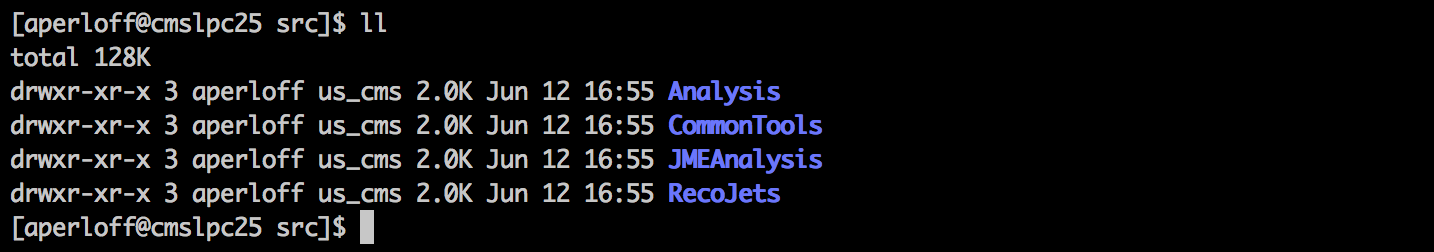
\includegraphics[width=\textwidth]{images/setup_software}
			\label{fig:setup_software}
		\end{figure}
	\end{textblock}

\end{frame}

%---------------------------------------------------------------------------------------------------------------------------------------
\begin{frame}[fragile]
	\frametitle{Exercise 1}
	\framesubtitle{pat::jets}

\begin{Verbatim}[label={Exercise 1}]
# Run with AODSIM + jetToolbox
# Run with MiniAODSIM + jetToolbox
# Run with MiniAODSIM + PAT
# In all of these cases you don't need to worry about double correcting
#     because you're reclustering jets and don't already have any corrections
\textcolor{Orange}{cmsRun jmedas_treeMaker.py}
\end{Verbatim}

\begin{block}{}
	\begin{itemize}
		\item Try playing around with the \textbf{doMiniAOD} and \textbf{doJetToolbox} options
		\item Change the jet collections and the correction levels
		\item \textbf{Hint}: For no corrections it seems you need to include just the L3Absolute corrections
		\item Explor the trees you make with this program
	\end{itemize}
\end{block}

\end{frame}

%---------------------------------------------------------------------------------------------------------------------------------------
\begin{frame}[fragile]
	\frametitle{Exercise 2}
	\framesubtitle{Uncorrect and recorrect jets from MiniAOD}

\begin{Verbatim}[label={Exercise 2}]
# You need to worry about double correcting if you are grabbing jets
#     from MiniAODSIM file directly
\textcolor{Orange}{git-cms-addPkg PhysicsTools/PatAlgos}
\textcolor{Orange}{cd PhysicsTools/PatAlgos/test/}
\textcolor{Orange}{cmsRun update_jets_from_MiniAOD.py}
\end{Verbatim}

\begin{block}{}
	\begin{itemize}
		\item Take a look at \href{https://github.com/cms-sw/cmssw/pull/8288}{https://github.com/cms-sw/cmssw/pull/8288}
		\item Explor the output of the program
	\end{itemize}
\end{block}

\end{frame}

%---------------------------------------------------------------------------------------------------------------------------------------
\begin{frame}[fragile]
	\frametitle{Exercise 3}
	\framesubtitle{Jet corrections on-the-fly}

\begin{Verbatim}[label={Exercise 3}]
\textcolor{Orange}{cmsRun jmedas_fwlite.py}
\end{Verbatim}

\begin{block}{}
	\begin{itemize}
		\item Take a look at the code and identify the lines which specify the JEC
		\item If you run over the same file and with the same set of JEC do your jets end up being the same?
	\end{itemize}
\end{block}

\end{frame}

%---------------------------------------------------------------------------------------------------------------------------------------
\begin{frame}[fragile]
	\frametitle{Exercise 4}
	\framesubtitle{reco::jets (AODSIM $+$ PFBRECO)}

\begin{Verbatim}[label={Exercise 4}]
# Run with AODSIM + PFBRECO
# not much worry about double correcting because AODSIM jets, or reclustered jets,
#     beacuse you do not have corrections already applied
\textcolor{Orange}{cd CMSSW_7_4_2_patch1/src/}
\textcolor{Orange}{git clone git@github.com:cms-jet/JetMETAnalysis.git}
\textcolor{Orange}{scram b -j 8}
\textcolor{Orange}{cd JetMETAnalysis/JetAnalyzers/test/}
\textcolor{Orange}{cmsRun run_JRA_cfg.py}
\end{Verbatim}

\begin{block}{}
	\begin{itemize}
		\item This is the same code we have been using to make the MC-truth corrections
		\item We will be moving to the JMEValidator code, which uses the JetToolbox
		\item This is a good example of both PFBRECO
		\item You can also look at bin/jet\_correction\_analyzer\_x.cc if you need another example of correcting jets on-the-fly
		\item Code located at \href{https://github.com/cms-jet/JetMETAnalysis}{https://github.com/cms-jet/JetMETAnalysis}
	\end{itemize}
\end{block}

\end{frame}

%---------------------------------------------------------------------------------------------------------------------------------------
\begin{frame}[fragile]
	\frametitle{Exercise 5}
	\framesubtitle{Jet Energy Resolution (JER) \& Uncertainties}

\begin{Verbatim}[label={Exercise 5}]
# Go back to jmedas_treeMaker.py and turn on either JER, uncertainties, or both
# JER also has the option to scale 1 sigma up or down from the nominal values
\textcolor{Orange}{cmsRun jmedas_treeMaker.py}
\end{Verbatim}

\begin{block}{}
	\begin{itemize}
		\item The JER factors are taken from \href{https://twiki.cern.ch/twiki/bin/view/CMS/JetResolution#JER_Scaling_factors_and_Uncertai}{https://twiki.cern.ch/twiki/bin/view/CMS/JetResolution\#JER\_Scaling\_factors\_and\_Uncertai}
		\item Because we have no data these have not been updated with $13\unit{TeV}$ resolution factors
	\end{itemize}
\end{block}

\end{frame}



